\section{Internacionalização}

Internacionalizar aplicações é cada vez mais uma tarefa comum em um desenvolvimento para web e é um dos processos importantes para o aumento da acessibilidade do sistema. O \texttt{framework} deve permitir mecanismo para facilitar a utilização de diversas línguas. Para tal, foi construido um conjunto de ferramentas para facilitar esse processo. A maioria dos frameworks web tem a sua maneira particular de prover esse mecanismo, mas o que muita gente desconhece é que existe uma forma padrão de fazer isso, definida na especificação do Java EE, através da JSP Standard TagLibs.

O MDArte utiliza esse mecanismo e já provê ela configurada. Assim, a especificação de novas linguas se torna uma tarefa ainda mais fácil.

Segue abaixo os passos para a definições de novas linguas.

\subsection{Mensagens}

Cada arquivo properties conterá todas as traduções do sistema. Todos os textos
do sistemas serão representados por uma \texttt{key}. Cada \texttt{key} e sua
respectiva mensagem, ou seja, \texttt{label} serão listadas em cada arquivo como
properties. Abaixo segue um exemplo:

\begin{lstlisting}[language=xml, frame=single, breaklines=true]
	label.key=Mensagem
\end{lstlisting}

Todas os recursos modelados no diagrama de atividades serão gerados com uma \texttt{key}.
Caso essa \texttt{key} não esteja no arquivo properties, o sistema utilizará a
\texttt{key} como \texttt{label} contudo sem o ponto.

Cada uma das possibilidades será abordada a seguir.

\subsubsection{Título de uma Página}

Todo título de página é gerado com uma key para o desenvolvedor possa definir no
custom-resources. 

\begin{lstlisting}[language=html, frame=single, breaklines=true]
	<tiles:put name="title" type="string">
    	<bean:message key="pagina.exemplo.title"/>
	</tiles:put>
\end{lstlisting}

\subsubsection{Campo ou Botão de uma Página}

Todo campo ou botão é gerado com uma key definida pelo o nome do caso de uso
somado com o nome do campo/botão. Segue abaixo um exemplo.

\begin{lstlisting}[language=html, frame=single, breaklines=true]
	<td class="field">
	<s:set name="__value" value="#session.form.nome"/>
	<div id="divnomeConsultaCursoUC" class="textfield field">
    	<label class="textfieldLabel" for="nome"><bean:message key="consulta.curso.uc.preencha.campos.consulta.curso.param.nome"/></label>
    	<s:textfield id="nomeConsultaCursoUC" name="nome" label="%{getText('consulta.curso.uc.preencha.campos.consulta.curso.param.nome')}" value="%{#session.form.nome}" title="" styleId="consultaCursoNome" />
</div>
\end{lstlisting}

\subsubsection{Exception}

Toda mensagem carregando uma \texttt{exception} também é substituída quando a
\texttt{key} na \texttt{exception} é encontrada no \texttt{custom-resource}.
Segue abaixo um exemplo.

\begin{lstlisting}[language=java, frame=single, breaklines=true]
	throw new Exception("ocorre.erro.esperado");

	throw new Exception("ocorre.erro.nao.esperado", exception);
\end{lstlisting}

Existem algumas funções que não interrompem a execução, mas possui o mesmo
efeito da \texttt{exception}. Segue abaixo um exemplo.

\begin{lstlisting}[language=java, frame=single, breaklines=true]
	saveErrorMessage(request, "informando.erro.key"); //Struts 1
	saveWarningMessage(request, "informando.aviso.key"); //Struts 1
	saveSuccessMessage(request, "informando.sucesso.key"); //Struts 1
	saveErrorMessage("informando.erro.key", container); //Struts 2
	saveWarningMessage("informando.aviso.key", container); //Struts 2
	saveSuccessMessage("informando.sucesso.key", container); //Struts 2
\end{lstlisting}

A função \texttt{saveErrorMessage} gera a seguinte mensagem na página:

\begin{figure}[H]
	\centering
	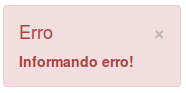
\includegraphics[scale=0.75]{files/imgs/internacionalizacao-00.png}
	\caption{Mensagem de erro}
	\label{mensagem_erro}
\end{figure}

\subsubsection{Passagem de Parâmetros}

Existe a possibilidade de passar parâmetros para a mensagem. Será passando um
\texttt{array} de \texttt{string} e na mensagem existirá marcadores informando
onde será colocado o conteúdo do \texttt{array}.

\textbf{Exemplo:}

\texttt{custom-resources.properties}

\begin{lstlisting}[language=xml, frame=single, breaklines=true]
	label.key=Mensagem com parametro {0}
\end{lstlisting}

\texttt{Código:}

\begin{lstlisting}[language=java, frame=single, breaklines=true]
	String[] parametro = new String[1];
	parametro[0] = "param1";
	saveErrorMessage("label.key", parametro, container); //Struts 2
	//saveErrorMessage(request, "label.key", parametro); //Struts 1
\end{lstlisting}

Assim será exibido a mensagem \texttt{Mensagem com
parametro param1} na figura abaixo:

\begin{figure}[H]
	\centering
	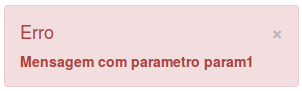
\includegraphics[scale=0.75]{files/imgs/internacionalizacao-01.png}
	\caption{Mensagem de erro com parâmetros}
	\label{mensagem_erro_parametro}
\end{figure}

\subsection{Arquivo de Configurações}

Para dar suporte a diversas linguas é necessário criar um arquivo com as \texttt{keys} do sistema para cada lingua e adicionar algumas configurações no \texttt{struts}. O \texttt{framework} MDARrte configura automaticamente o \texttt{struts} para facilitar o desenvolvedor nessa tarefa. Para tal, edite o arquivo \textbf{<DiretorioProjeto>}/mda/conf/andromda.xml e na propriedade \texttt{languages} informe os locales que serão utilizados.

Exemplo:

\begin{lstlisting}[language=xml, frame=single, breaklines=true]
	<property name="languages">pt,en,fr</property>
\end{lstlisting}

Após a geração utilizando essa configuração será criado novos três arquivos: 

\begin{lstlisting}[language=xml, frame=single, breaklines=true]
	custom-resources_en.properties
	custom-resources_pt.properties
	custom-resources_fr.properties
\end{lstlisting}

Além do arquivo já criado no geração da aplicação:

\begin{lstlisting}[language=xml, frame=single, breaklines=true]
	custom-resources.properties
\end{lstlisting}

Automaticamente o sistema irá detectar qual locale do browser que o usuário está
utilizando e utilizará o locale correto. Caso não exista o locale pré-definido,
o sistema utilizará o \texttt{custom-resources} padrão.

O desenvolvedor poderá forçar um locale específico pelo código. Exemplo: 

\begin{lstlisting}[language=java, frame=single, breaklines=true]
	//Recuperando o Locale
	Locale locale = (Locale) request.getSession().getAttribute("org.apache.struts.action.LOCALE");

	//Definindo um Locale
	request.getSession().setAttribute("org.apache.struts.action.LOCALE", new Locale("pt", "BR"));
\end{lstlisting}
